% Created 2023-04-13 Thu 14:26
% Intended LaTeX compiler: pdflatex
\documentclass{report}
                              \usepackage[utf8]{inputenc}
\usepackage[T1]{fontenc}
\usepackage{RJournal}
\usepackage{amsmath,amssymb,array}
\usepackage{booktabs}
\sectionhead{Contributed research article}
\volume{XX}
\volnumber{ZZ}
\year{20YY}
\month{MM}
\usepackage{blindtext}
\usepackage{xcolor}
\usepackage{listings}
\usepackage{hyperref}
\hypersetup{colorlinks=true, linkcolor=blue, filecolor=magenta, urlcolor=cyan}
\usepackage{float}
\DeclareMathOperator*{\argmax}{argmax}
\DeclareMathOperator*{\argmin}{argmin}
\newcommand{\J}{\ensuremath{J}}
\newcommand{\1}{\ensuremath{\mathbf{1}}}
\newcommand{\h}{\ensuremath{\lambda}}
\newcommand{\indep}{\ensuremath{\perp\hspace*{-1.4ex}\perp}}
\newcommand{\T}{\ensuremath{\widetilde{T}}}
\newcommand{\X}{\ensuremath{{W}}}
\renewcommand{\t}{\ensuremath{\Tilde{t}}}
\newcommand{\ax}{\ensuremath{\mid a,\,{w}}}
\newcommand{\aX}{\ensuremath{\mid A = a,\,{W}}}
\newcommand{\AX}{\ensuremath{\mid A,\,{W}}}
\newcommand{\x}{\ensuremath{{w}}}
\newcommand{\trt}{\ensuremath{\pi^*}}
\newcommand{\tk}{\ensuremath{t_{k}}}
\newcommand{\lj}{\ensuremath{l}}
\newcommand{\jj}{\ensuremath{j}}
\newcommand{\tK}{\ensuremath{K}}
\newcommand{\tKi}{\ensuremath{k}}
\newcommand{\TK}{\ensuremath{\mathcal{T}}}
\newcommand{\g}{\ensuremath{\pi}}
\renewcommand{\L}{\ensuremath{W}}
\renewcommand{\l}{\ensuremath{w}}
\newcommand{\tDelta}{\ensuremath{\widetilde{\Delta}}}
\newcommand{\F}{\ensuremath{\mathcal{F}}}
\setcounter{secnumdepth}{5}
\newcommand{\tildelambda}{\tilde{\lambda}}

\lstset{
keywordstyle=\color{blue},
commentstyle=\color{red},stringstyle=\color[rgb]{0,.5,0},
literate={~}{$\sim$}{1},
basicstyle=\ttfamily\small,
columns=fullflexible,
breaklines=true,
breakatwhitespace=false,
numbers=left,
numberstyle=\ttfamily\tiny\color{gray},
stepnumber=1,
numbersep=10pt,
backgroundcolor=\color{white},
tabsize=4,
keepspaces=true,
showspaces=false,
showstringspaces=false,
xleftmargin=.23in,
frame=single,
basewidth={0.5em,0.4em},
}
\renewcommand*\familydefault{\sfdefault}
\itemsep2pt
\author{imbroglio}
\date{\today}
\title{}
\begin{document}

\title{concrete R Paper: Title TBD}
\subtitle{}
\author{by David Chen, Thomas Gerds, Helene Rytgaard, Maya L. Petersen, Mark van der Laan, ...}

\maketitle

\abstract{
% Competing risks are a common but under-addressed feature in biomedical survival studies. This article outlines a causal inference workflow that illuminates whether or not the researchers' question of interest involves competing risks and introduces the R package \CRANpkg{concrete} which implements a targeted maximum likelihood estimator for the cause-specific absolute risks for time-to-event outcomes measured in continuous or near-continuous time. The package can be used for survival analyses with or without competing risks and allows users to estimate causally-interpretable estimands such as risk ratios and risk differences using possibly misspecified cause-specific Cox models. Point estimates can be produced using G-formula plug-in or TMLE, and influence curve-based asymptotic inference will be provided for TMLE. For target estimands involving multiple times or events, simultaenous confidence bands can be produced using nfluence curve-based simulation. This paper will demonstrate the use of \CRANpkg{concrete} using the PBC dataset.

This article introduces the R package \CRANpkg{concrete} which implements a recently developed targeted maximum likelihood-based estimator (TMLE) targeting the cause-specific absolute risks of time-to-event outcomes measured in continuous time. This package can be used to estimate the effects of static and dynamic interventions on a binary treatment given at baseline, quantified as causally-interpretable absolute risks, risk differences, and risk ratios. Cause-specific hazards are estimated by cross-validated Super Learner ensembles of Cox regressions, which are then used to compute g-formula plug-in and TMLE point estimates of absolute risks. Influence curve-based asymptotic inference is provided for TMLE estimates and simultaneous confidence bands can be computed for target estimands that span multiple multiple times or events. In this paper we review one-step continuous-time TMLE methodology as it is situated in the larger causal inference targeted learning workflow, describe how it is implemented in \CRANpkg{concrete}, and demonstrate its use on the PBC dataset.
}

\section{Introduction}
\label{intro}
In biomedical survival applications, study subjects are often susceptible to competing risks such as all-cause mortality. In recent decades, several competing risk methods have been developed; including the Fine-Gray (\cite{fine_proportional_1999}), pseudovalue (\cite{klein_regression_2005}), and direct binomial (\cite{scheike_predicting_2008}, \cite{gerds_absolute_2012}) regressions; and authors have consistently cautioned against the use of standard survival estimands for causal questions involving competing risks. Nevertheless, reviews of clinical literature by \cite{koller_competing_2012} and \cite{austin_accounting_2017} found that most trials still fail to adequately address the effect of potential competing risks in their studies. Meanwhile, formal causal inference frameworks (\cite{holland_statistics_1986}, \cite{pearl_causal_2016}) have gained recognition for their utility in translating clinical questions into statistical analyses and the targeted maximum likelihood estimation (TMLE) (\cite{laan_targeted_2011}, \cite{laan_targeted_2018}) methodology developed from the estimating equation and one-step estimator lineage of semi-parametric efficient methods based on solving efficient influence curves (EICs). The targeted learning roadmap (\cite{petersen_causal_2014}) combines these developments into a cohesive causal inference workflow and provides a structured way to think about statistical decisions. In this paper we apply the targeted learning roadmap to an analysis of time-to-event outcomes and demonstrate the R package \CRANpkg{concrete}, which implements a recently developed continuous-time TMLE targeting cause-specific absolute risks (\cite{rytgaard_estimation_2021}, \cite{rytgaard_one-step_2021}).

\CRANpkg{concrete} (\textbf{con}tinuous-time \textbf{c}ompeting \textbf{r}isks \textbf{e}stimation using \textbf{T}ML\textbf{E}) can, given identification and regularity assumptions, be used to efficiently estimate the treatment effect of interventions given at baseline. \cite{rytgaard_one-step_2021} provides a rigorous explanation of this method and the necessary assumptions for causal identification, but in short the implemented one-step TMLE procedure consists of two stages: 1) an initial estimation of nuisance parameters and 2) a targeted update of the initial estimators to solve the EIC of the target statistical estimand (\cite{laan_unified_2003-1}, \cite{kennedy_semiparametric_2016}). In \CRANpkg{concrete} this initial nuisance parameter estimation is performed using Super Learning, a cross-validated machine learning ensemble algorithm with asymptotic oracle guarantees (\cite{laan_unified_2003}, \cite{laan_super_2007}, \cite{polley_superlearner_2021}). When data-generating mechanisms are unknown, Super Learners with robust candidate libraries and appropriate loss functions often give users the best chance of achieving the convergence rates needed for TMLE's asymptotic properties. The subsequent targeted update is based in semi-parametric efficiency theory; specifically that efficient regular and asymptotically linear (RAL) estimators must have influence curves equal to the efficient influence curve (EIC) of the target statistical estimand (\cite{laan_targeted_2011}, \cite{kennedy_semiparametric_2016}). This TMLE update shfits the initial nuisance parameter estimates to solve target EICs, thus recovering normal asymtotic inference even while leveraging the power of flexible machine-learning algorithms for initial estimation. In Section \ref{cv} we outline how Super Learner is used to estimate nuisance parameters in \CRANpkg{concrete} while more detailed guidance on how to best specify Superlearner estimators is provided in \cite{phillips_practical_2022}. Section \ref{EIC} details the subsequent targeted update, with a full description provided in \cite{rytgaard_one-step_2021}. 

Currently \CRANpkg{concrete} can be used for estimands derived from cause-specific absolute risks, such as risk ratios and risk differences, under static and dynamic interventions on binary treatments given at baseline. Estimands can be jointly targeted at multiple times, up to full risk curves over an interval, and for multiple events in cases with competing risks. Methods are available to handle right-censoring, competing risks, and confounding by baseline covariates. Point estimates can be computed using g-formula plug-in or one-step TMLE, and asymptotic inference for the latter is derived from the variance of the efficient influence curve (EIC). 

\CRANpkg{concrete} is not meant to be used for left trunctation (i.e. delayed entry), interval censored data, or clustered data. Currently the Super Learners for estimating conditional hazards must be comprised of Cox regressions though the incorporation of penalized Cox (coxnet) and hazard estimators based on highly adaptive lasso (HAL) are planned in future package versions. Support for stochastic interventions or interventions on multinomial and continuous treatments and support for longitudinal methods to handle time-dependent treatments (e.g. drop-in) and time-dependent confounding are in longer term development.

\subsection{A concrete Example: Competing Risks Analysis of the PBC Dataset}
\label{nutshell}
\lstset{language=r,label=pbc nutshell,caption= ,captionpos=b,numbers=none,otherkeywords={}, deletekeywords={}}
\begin{lstlisting}
# Prepare Data
library(concrete)
data <- survival::pbc[, c("time", "status", "trt", "age", "sex", "albumin")]
data <- subset(data, subset = !is.na(data$trt))
data$trt <- data$trt - 1

# Specify Analysis
ConcreteArgs <- formatArguments(DataTable = data,
				EventTime = "time",
				EventType = "status",
				Treatment = "trt",
				Intervention = 0:1,
				TargetTime = 90 * (6:30))

# Compute
ConcreteEst <- doConcrete(ConcreteArgs)

# Return Output
ConcreteOut <- getOutput(ConcreteEst, Estimand = "RD", Simultaneous = FALSE)
plot(ConcreteOut, ask = FALSE)
\end{lstlisting}

\begin{figure}[H]
\center
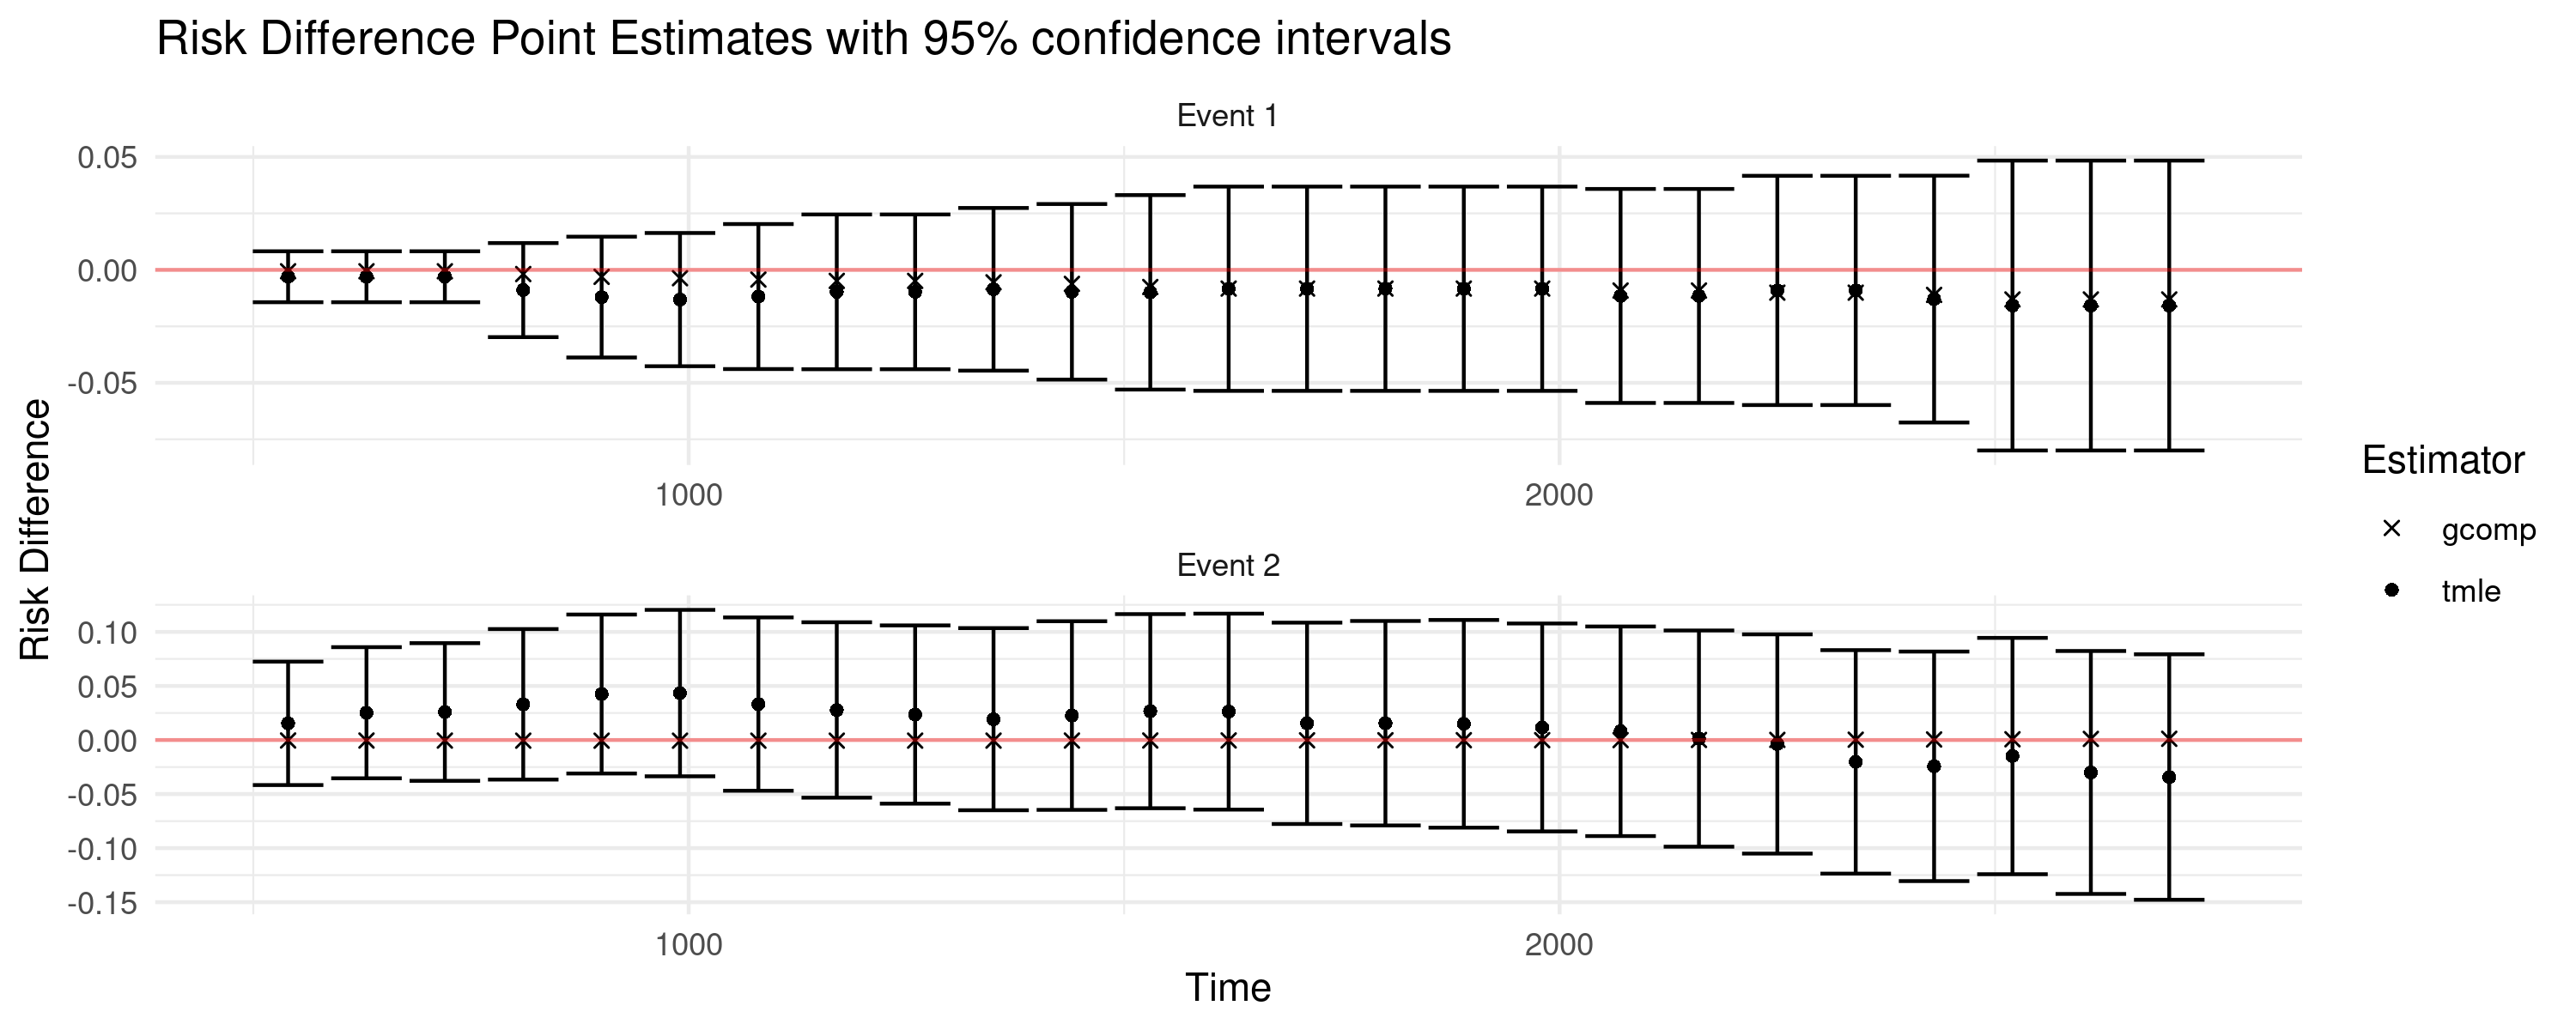
\includegraphics[width=\linewidth]{fig/RD.png}
\end{figure}

\subsection{Other packages}
\label{otherpkgs}
\CRANpkg{concrete} is the first R package for general use implementing a continous-time TMLE, but several existing packages implement discrete-time TMLEs for survival estimands; namely \CRANpkg{ltmle} (\cite{schwab_ltmle_2020}), \CRANpkg{stremr} (\cite{sofrygin_stremr_2017}), and \CRANpkg{survtmle} (\cite{benkeser_survtmle_2019}). These packages either natively or can be adapted to perform TMLE for absolute risks of right-censored survival or competing risks estimands; \CRANpkg{ltmle} and \CRANpkg{stremr} use the method of iterated expectations while \CRANpkg{survtmle} can target the hazard-based survival formulation. Notably these packages all operate in discrete-time and would require discretization of continuous-time data which can negatively impact estimator performance.

As for existing continuous-time survival estimation packages, \CRANpkg{concrete} adds a TMLE method to a small number of packages implementing semi-parametric efficient survival estimators. The \ctv{Causal Inference} CRAN Task View lists \CRANpkg{riskregression} (\cite{gerds_riskregression_2022}) as estimating treatment effect estimands in survival settings. \CRANpkg{riskregression} implements the IPTW and double-robust AIPTW estimators as well as a g-formula plug-in. None of the packages listed on the \ctv{Survival} CRAN Task View are described as implementing efficient semi-parametric estimators for survival estimands, though available via Github are the R packages \href{https://github.com/RobinDenz1/adjustedCurves}{adjustedCurves} (\cite{denz_comparison_2022}) and \href{https://github.com/tedwestling/CFsurvival}{CFsurvival} (\cite{westling_inference_2021}), which implement the AIPTW and a cross-fitted doubly-robust estimator respectively.

\subsection{Structure of this manuscript}
\label{sec:org875f4d5}
This article is written for readers wishing to use the \CRANpkg{concrete} package for their own analyses and for readers interested in an applied introduction to the one-step continuous-time TMLE method described in \cite{rytgaard_one-step_2021}. Section \ref{concepts} outlines the targeted learning approach to time-to-event causal effect estimation, with subsection \ref{estimation} providing details on our one-step TMLE implementation. Usage of the \CRANpkg{concrete} package and its features is then provided in Section \ref{UsingConcrete}, using the example of a simple competing risks analysis of the PBC dataset. 


\section{Theoretical Framework}
\label{concepts}
\subsection{The Targeted Learning Roadmap}
\label{TLRoadmap}
At a high level, the targeted learning roadmap for analyzing continuous-time survival or competing risks consists of:
\begin{enumerate}
  \item Specifying the causal model and defining a causal estimand (e.g. causal risk difference). Considerations include defining a time zero and time horizon, specifying the intervention (i.e. treatment) variable and the desired intervention(s), and specifying the target time(s) and event(s) of interest.
  \item Defining a statistical model and statistical estimand, and evaluating the assumptions necessary for the statistical estimand to identify the causal estimand. Considerations include identifying confounding and right-censoring variables, establishing positivity for desired interventions, and formalizing knowledge about the statistical model (e.g. dependency structures or functional structures such as proportional hazards).
  \item Performing estimation and providing inference. Considerations include prespecification to avoid misleading inference, selecting an estimator with desirable theoretical properties (e.g. consistency and efficiency within a desired class), and assessing via outcome-blind simulations the estimator's robustness and suitability for the data at hand.
\end{enumerate}

In the following sections we discuss these three stages in greater detail.

\subsection{The Causal Model: Counterfactuals, Interventions, and Causal Estimands}
\label{CausalData}
With time-to-event data, typical counterfactual outcomes are how long it would take for some events to occur if subjects were hypothetically to receive some intervention. Let \(A\) be this intervention variable and let \(d\) be the intervention rule, i.e. the function that assigns values to \(A\). The simplest interventions are static rules setting \(A\) to some value \(a\) in the space of treatment values \(\mathcal{A}\), while more flexible dynamic treatment rules might assign treatments based on subjects' baseline covariates, and stochastic treatment rules can incorporate randomness and may even depend on the natural treatment assignment mechanism in so-called modified treatment policies. No matter the type of intervention, if we let \(d\) represent the intervention rule then the associated counterfactual survival data \(X \sim P^d\) might take the form
\begin{equation}
 X = \left(T^d,\, \Delta^d,\, A^d, \L \right) \label{causaldata}
\end{equation}
where \(T^d \in (0, t_{max}]\) is earliest occurence of any of the \(J\) events under intervention \(d\), \(\Delta^d \in \{1, \dots, J\}\) shows which of the \(J\) events occured first under intervention \(d\), and \(A^d\) is the treatment value that would be assigned under intervention \(d\). Notably, we do not include censoring in this counterfactual data and instead isolate just those events that experimenters would like to observe in their ideal hypothetical experiment. For ideal experiments tracking just one event, the causal setting is one of classic survival; if instead mutually exclusive events would be allowed to compete, then the causal setting is one with competing risks. 

With the counterfactual data defined, causal estimands can then be specified as functions of the counterfactual data. For instance, if we were interested in effects of interventions \(d_0\) versus \(d_1\) on time-to-event outcomes, the counterfactual data \(\tilde{X} \sim P^{\,0,1}\) might be represented as
\begin{align*}
\tilde{X} = \left(T^{d_0},\, \Delta^{d_0},\, A^{d_0}, T^{d_1},\, \Delta^{d_1},\, A^{d_1}, \L \right)
\end{align*}
We could then define estimands such as the causal event \(j\) relative risks at time \(t\) 
\begin{align}
\Psi_{F_{j,t}}(P^{\,0,1}) &= \frac{{P}(T^{d_1} \leq t, \Delta^{d_1} = j)}{{P}(T^{d_{0}} \leq t, \Delta^{d_{0}} = j)}
\label{causalrisk}
\end{align}
These estimands may be of interest at a single timepoint or at many, including full curves over a time interval (\(\Psi_{F_{j,t}}(P^{\,0,1}) : t \in (0, t_{max}]\)), and in the case of competing risks may involve multiple events (\(\Psi_{F_{j,t}}(P^{\,0, 1}) : j \in 1, \dots, J\)). In any case, once the desired causal quantity of interest has been expressed as a function of the counterfactual data, efforts can then be made to identify the causal estimand with a function of observed data, i.e. a statistical estimand.

\subsection{Observed Data, Identification, and Statistical Estimands}
\label{ObservedData}
Observed time-to-event data \(O \sim P_0\) with \(J\) competing events can be represented as:
\begin{equation}
 O = \left(\T,\, \tDelta,\, A,\, \L \right) \label{obs-data}
\end{equation}
where \(\T \in (0, t_{max}]\) is the earlier of the first event time \(T\) or the right-censoring time \(C\), \(\tDelta \in \{0, \dots, J\}\) indicates which event occurs (with 0 indicating right-censoring), \(A\) is the observed treatment and \(\L\) is the set of baseline covariates.

To link causal estimands such as Eq. \eqref{causalrisk} to statistical estimands, we need a set of untestable identification assumptions to hold: consistency, positivity, no unmeasured confounding, and conditionally independent censoring. Readers can find a full discussion of these identification assumptions for absolute risk estimands in Section 3 of \cite{rytgaard_continuous-time_2021}. Given these assumptions, we can identify the cause-\(j\) absolute risk at time \(t\) under intervention \(d\) using the g-computation formula as
\begin{equation}
P(T^d \leq t, \Delta^d = j) = \mathbb{E}_{\mathcal{\L}} \left[ \int_{\mathcal{A}} \,  F_j(t \ax) \, \g^* (a \mid \l) \, da \right] \label{absrisk}
\end{equation}
where \(\g^*(a \mid \l)\) is the treatment propensity implied by the intervention \(d\) and \(F_j(t \ax)\) is the conditional cause-\(j\) absolute risk
\begin{equation*}
F_j(t \ax) = \int_0^t \lambda_j(s \ax) \, S(s\texttt{-} \ax) \, ds 
\end{equation*}
with the cause-\(j\) conditional hazard
\begin{equation*}
\lambda_j(t \ax) = \lim\limits_{h \to 0} \frac{1}{h} P(\T \leq t + h,\, \tDelta = j \mid \T \geq t,\, a,\, \x)
\end{equation*}
and conditional event-free survival
\begin{equation}
S(t \ax) = \exp\left(-\int^{t}_{0} \sum\limits_{j=1}^{J} \lambda_j(s \ax) \, ds \right) \label{evfreesurv}
\end{equation}
From Eq \eqref{absrisk}, it follows that we can identify the causal cause-\(j\) relative risk \eqref{causalrisk} at time \(t\) by
\begin{equation}
\Psi_{F_{j,t}}(P_0) = \frac{\mathbb{E}_{\mathcal{\L}} \left[ \int_{\mathcal{A}} \,  F_j(t \ax) \, \g^*_{d_1} (a \mid \l) \, da \right]}{\mathbb{E}_{\mathcal{\L}} \left[ \int_{\mathcal{A}} \,  F_j(t \ax) \, \g^*_{d_0} (a \mid \l) \, da \right]} \label{obsrisk}
\end{equation}
where \(\g^*_{d_0}\) and \(\g^*_{d_1}\) represent the treatment propensities implied by treatment rules \(d_0\) and \(d_1\) respectively.

It should be noted that even without the identification assumptions for causal inference, statistical estimands such as Eq. \eqref{obsrisk} may still have valuable interpretations as standardized measures isolating the importance of the "intervention" variable (\cite{laan_statistical_2006}).

\subsection{Targeted Estimation}
\label{estimation}
The TMLE procedure for estimands derived from cause-specific absolute risks begins with estimating the treatment propensity \(\g\), the conditional hazard of censoring \(\lambda_c\) and the conditional hazards of events \(\lambda_j \,:\; j = 1, \dots, J\). In \CRANpkg{concrete} these nuisance parameters are estimated using the Super Learner algorithm, which involves specifying a cross-validation scheme, compiling a library of candidate algorithms, and designating a cross-validation loss function and a Super Learner meta-learner.

\subsubsection{Specifying Super Learners}
\label{cv}
For a simple \(V\text{-fold}\) cross validation setup, let 
\(Q_n = \{O_i\}_{i=1}^n \sim P_n\) 
be the observed \(n\) i.i.d observations of \(O \sim P_0\) and let
\(B_n \in \{1, ... , V\}^n\)
be a random vector that assigns the \(n\) observations into \(V\) validation folds. Then for each \(v\) in \(1, ..., V\) we define a training set 
\(Q^\mathcal{T}_v = \{O_i : B_n^i = v\} \sim  P^\mathcal{T}_v\)
and corresponding validation set
\(Q^\mathcal{V}_v = \{O_i : B_n^i \neq v\} \sim P^\mathcal{V}_v\).

Having specified a cross-validation scheme, the next steps are to construct the Super Learner candidate library, define an appropriate loss function, and select a Super Learner meta-learner. Super Learner libraries should be comprised of candidate algorithms that range in flexibility while respecting existing data-generating knowledge. For instance, candidate estimators should incorporate covariates and interactions known to be predictive of outcomes, and if the number of independent observations \(n\) is much greater than the number of covariates, then more highly flexible candidate algorithms such as Highly Adaptive Lasso (HAL) should be included in the Super Learner library. If on the other hand the number of covariates approaches \(n\), then libraries should be comprised of fewer and less flexible candidate algorithms, potentially with native penalization as with coxnet or by pairing candidate regression algorithms with screening algorithms. It should be noted that using HAL for initial nuisance parameter estimation can achieve the neceesary convergence rates (\cite{laan_generally_2017,benkeser_highly_2016,rytgaard_continuous-time_2021}) for TMLE to be efficient. Super Learner loss functions should imply a risk that is minimized by the true data-generating process and define a loss-based dissimilarity tailored to the target parameter and for maximal robustness the discrete selector that simply selects the best performing candidate should be used as the Super Learner meta-learner. For more flexibility, Super Learners using more flexible meta-learner algorithms can be nested as candidates within a larger Super Learner, and additional guidance is provided in \cite{laan_super_2007} and Chapter 3 of \cite{laan_targeted_2011}.

Currently the default cross-validation setup in \CRANpkg{concrete} generally follows the guidelines laid out in \cite{phillips_practical_2022}, with the number of cross-validation folds increasing with smaller sample sizes. Default Super Learner libraries are provided and will be detailed in the following sections, but should be amended to suit the data at hand and to incorporate subject matter knowledge.

\subsubsection{Estimating Treatment Propensity}
\label{trtps-est}
For estimating the treatment propensity let \(\g_0\) be the true conditional distribution of \(A\) given \(\X\), let
\(\mathcal{M}_{\g} = \left\{\Hat{\g} : P_n \to \Hat{\g}(P_n)\right\}\)
be the library of candidate propensity score estimators, and let \(L_\g\) be a loss function such that the risk \(\mathbb{P}_0\,L_\g(\g) \equiv \mathbb{E}_0\left[L_\g(\g, O)\right]\) is minimized by \(\g_0\). The discrete Super Learner estimator is then the candidate propensity estimator with minimal cross validated risk, 
\begin{equation}
\Hat{\g}^{SL} = \argmin_{\Hat{\g} \in \mathcal{M}_\g} \sum_{v = 1}^{V} \mathbb{P}_{Q^\mathcal{V}_v} \; L_\g(\Hat{\g}(P^\mathcal{T}_v)) \label{propsl}
\end{equation}
where \(\Hat{\g}(P^\mathcal{T}_v)\) are candidate propensity score estimators trained on data \(Q^\mathcal{T}_v\). Currently \CRANpkg{concrete} uses the default \CRANpkg{SuperLearner} loss functions and specifies a default library consisting of glmnet and xgboost.

\subsubsection{Estimating Conditional Hazards}
\label{haz-est}
For \(\delta = 0, \dots, J\) where (\(\delta = 0\)) is censoring and (\(\delta \in \{1, \dots, J\}\)) are outcomes of interest, let \(\lambda_{\delta} \,:\; \delta = 0, \dots, J\) be the true conditional hazards, let \(\mathcal{M}_\delta = \{\Hat{\lambda}_\delta : P_n \to \Hat\lambda_{\delta}(P_n)\}\) be the libraries of candidate estimators, and let \(L_{\delta}\) be loss functions such that the risks \(\mathbb{P}_0\,L_{\delta}(\cdot)\) are minimized by the true conditional hazards \(\lambda_{\delta}\). The discrete Super Learner selectors for each \(\delta\) then chooses the candidate which has minimal cross validated risk 
\begin{equation}
\Hat{\lambda}_\delta^{SL} = \argmin_{\Hat{\lambda}_\delta \in \mathcal{M}_\delta} \sum_{v = 1}^{V} \mathbb{P}_{Q^\mathcal{V}_v} \; L_{ \delta}(\Hat{\lambda}_{\delta}(P^\mathcal{T}_v)) \;:\; \delta = 0, \dots, J\label{hazsl}
\end{equation}
where \(\Hat{\lambda}_\delta(P^\mathcal{T}_v)\) are candidate event \(\delta\) conditional hazard estimators trained on data \(Q^\mathcal{T}_v\). The current \CRANpkg{concrete} default is a library of two Cox models, treatment-only and main-terms, with cross-validated risk computed using negative log Cox partial-likelihood loss
\[ \mathbb{P}_{Q^\mathcal{V}_v} \; L_{ \delta}(\Hat{\lambda}_{\delta}(P^\mathcal{T}_v)) =  \mathbb{P}_{Q^\mathcal{V}_v} \; L_{ \delta}(\Hat{\beta}_{\delta, Q^\mathcal{T}_v}) = - \sum_{i: \, O_i \in Q^\mathcal{V}_v} \left[\Hat{\beta}^{'}_{\delta, Q^\mathcal{T}_v}\,\L_i - \log\left[\sum_{h \in \mathcal{R}(\T_i)} \exp(\Hat{\beta}^{'}_{\delta, Q^\mathcal{T}_v}\,\L_h)\right]\right] \,\]
where \(\mathcal{R}(t)\) is the risk set at time \(t\), \(\{h \,:\, \T_h \geq t\}\) and \(\Hat{\beta}^{'}_{\delta, Q^\mathcal{T}_v}\) are the coefficients of an event \(\delta\) candidate Cox regression trained on data \(Q^\mathcal{T}_v\). 

\subsubsection{Solving the Efficient Influence Curve}
\label{EIC}
For parameters such as risk ratios which are derived from cause-specific absolute risks, we solve a vector of absolute risk EICs with one element for each combination of target event, target time, and intervention. That is, the EIC for a target parameter involving \(J\) competing events, \(K\) target times, and \(M\) interventions is a \(J \times K\times M\) dimensional vector where the component corresponding to the cause-specific risk of event \(\jj\), at time \(t_k\), and under intervention propensity \(\trt_{m}\) is:
\begin{align}
    D^*_{m, \jj, k}(\lambda, \g, S_c)(O) = \sum_{\lj = 1}^{J} \int \; &h_{m,\, \jj,\, k,\, \lj,\, s}(\lambda, \g, S_c)(O) \, \left(N_{\lj}(s) - \1(\T \geq s) \, \lambda_\lj(s \AX)\right) \, ds \label{eic} \\
    &{\color{blue!60!black}+ \int_{\mathcal{A}} F_\jj(t_k \mid A = a, \X)\,\trt_m(a \mid \X) \, da - \Psi_{\trt, \jj, t}(P_0)}  \nonumber 
\end{align}
where \(N_l : l = 0,\dots, J\) are the cause-specific counting processes
\[N_l(s) = \1\left\{\T \leq s, \tDelta = l\right\} \]
and \(h_{m,\, \jj,\, k,\, \lj,\, s}(\lambda, \g, S_c)(O)\) is the TMLE "clever covariate"
\begin{align}
    h_{m,\, \jj,\, k,\, \lj,\, s}&(\lambda, \g, S_c)(O) = \frac{{\color{blue}\trt_m(A \mid \X)\,} \1(s \leq t_k)}{{\color{green!70!black}\g(A \mid \X) \;S_c(s\text{-} \AX)}} \, \bigg(\1(\lj = \jj) - \frac{{\color{red}F_\jj(t_k \AX)} - {\color{red} F_\jj(s \AX)}}{{\color{red} S(s \AX)}}\bigg) \label{clevcov}
\end{align}
We highlight here that clever covariate is a function of the {\color{blue}intervention-defined treatment propensity}, the {\color{green!70!black}observed intervention-related densities} which are unaffected by TMLE targeting, and the {\color{red}observed outcome-related densities} which will be updated by TMLE targeting. Note also that notation for the EIC (\(D^*_{m, \jj, k}(\lambda, \g, S_c)(O)\)) and clever covariate (\(h_{m,\, \jj,\, k,\, \lj,\, s}(\lambda, \g, S_c)(O)\)) reflect their dependence on \(P\) through the outcome-related conditional hazards \(\lambda = (\lambda_l \;:\;  l = 1, \dots, J)\) and the intervention-related treatment propensity \(\g\) and conditional censoring survival \(S_c(t \ax) = \exp\left(-\int^{t}_{0} \lambda_0(s \ax) \, ds \right)\).

The one-step continuous-time survival TMLE involves updating the cause-specific hazards \(\lambda\) along the universally least favorable submodel, which is implemented as recursive limited updates along a sequence locally least favorable submodels. To describe this procedure, let us first introduce the following vectorized notation:
\begin{align*}
{D}^{*} &= \left(D^*_{m, \jj, k} : m = 1,\dots,M \,,\; \jj=1,\dots,J \,,\; k=1,\dots,K\right)\\
h_{\lj, s} &= \left(h_{m,\, \jj,\, k,\, \lj,\, s} : m = 1,\dots,M \,,\; \jj=1,\dots,J \,,\; k=1,\dots,K\right)
\end{align*}
The one-step continuous-time survival TMLE recursively updates the cause-specific hazards in the following manner: starting from \(b=0\), with \(\lambda^0_j = \hat{\lambda}^{SL}_j\), and \(\lambda^b = \left(\lambda^b_l \;:\; l = 1, \dots, J\right)\)
\begin{equation}
\lambda^{b+1}_{l} = \lambda^{b}_l \, \exp \left( \frac{\left<\mathbb{P}_n {D}^*( \lambda^b, \g,  S_c)(O),\; h_{j, s}( \lambda^b, \g,  S_c)(O) \right>}{|| \mathbb{P}_n {D}^*( \lambda^b, \g, S_c)(O)||} \; \epsilon_b\right), \quad l = 1,\dots,J \label{one-step}
\end{equation}

where
\begin{align*}
\left<x , y \right>& = x^\top y \hspace{.5cm}, \hspace{.5cm} ||x|| = \sqrt{x^\top x}
\end{align*}
and the step sizes \(\epsilon_b\) are chosen such that
\[|| \mathbb{P}_n {D}^*( \lambda^{b+1}, \g, S_c)(O)|| < || \mathbb{P}_n {D}^*( \lambda^{b}, \g, S_c)(O)||\]
The recursive update following Eq \eqref{one-step} is completed at the iteration \(B\) where
\begin{equation}
\mathbb{P}_n {D}^*( \lambda^B, \g, S_c)(O) \leq \frac{\sqrt{\mathbb{P}_n {D}^*( \lambda^B, \g, S_c)(O)^2}}{\sqrt{n} \, \log(n)} \label{one-step-stop}
\end{equation}
This updated vector of conditional hazards \(\lambda^B\) is then used to compute a plug-in estimate the target statistical estimand. 

\subsubsection{Estimating TMLE Variance}
\label{sec:org478189d}

In \CRANpkg{concrete}, the variance of TMLE estimates of targeted risks is estimated from the EIC's variance divided by the sample size, \(\frac{\mathbb{P}_n \;D^*( \lambda^B, \g, S_c)(O)^2}{n}\), which is a consistent estimator for the variance of asymptotically linear estimators. In the presence of significant positivity violations (which may be seen as propensity scores close to 0), this EIC-derived variance estimator will be anti-conservative and variance estimation by bootstrap may be more reliable. However, bias resulting from positivity violations cannot be remedied in this way, and so other methods of addressing positivity violations (\cite{petersen_diagnosing_2012}) are recommended instead. For multidimensional estimands, simultaneous confidence intervals can be computed by simulating the \(1 - \alpha\) quantiles of a multivariate normal distribution with the covariance structure of the estimand EICs.

\section{Using concrete}
\label{UsingConcrete}
The basic \CRANpkg{concrete} workflow consists of calling three functions in sequence: \code{formatArguments()}, \code{doConcrete()}, and \code{getOutput()}. Users specify their estimation problem and desired analysis through \code{formatArguments()}, which checks the specified analysis for red flags and then produces a \code{"ConcreteArgs"} environment object. The \code{"ConcreteArgs"} object is then passed into \code{doConcrete()} which performs the specified continuous-time one-step survival TMLE and produces a \code{"ConcreteEst"} object which can be interrogated for diagnostics and estimation details. The \code{"ConcreteEst"} object can then be passed into \code{getOutput()} to produce tables and plots of cause-specific absolute risk derived estimands such as risk differences and relative risks. 


\subsection{formatArguments()}
\label{formatArguments}

\subsection{ConcreteArgs}
\label{sec:orga5407eb}
The arguments of \code{formatArguments()} are primarily involved in specifying 1) the observed data structure, 2) the target estimand, or 3) the TMLE estimator. The output \code{"ConcreteArgs"} object is an environment containing these necessary elements of a continuous-time TMLE analysis.

\lstset{language=r,label= ,caption= ,captionpos=b,numbers=none,otherkeywords={}, deletekeywords={}}
\begin{lstlisting}
ConcreteArgs <- formatArguments(
  DataTable = data,
  EventTime = "time",
  EventType = "status",
  Treatment = "trt",
  Intervention = 0:1,
  TargetTime = 90 * (6:30),
  TargetEvent = 1:2,
  MaxUpdateIter = 500
)
\end{lstlisting}

\subsubsection{Data}
\label{ObservedDataConcrete}
Observed data is passed into the \code{DataTable} argument as either a \code{data.frame} or \code{data.table} object, which must contain columns corresponding to the observed time-to-event \(\T\), the indicator of which event occured \(\Delta\), and the treatment variable \(A\). Any number of columns containing baseline covariates \(\L\) can also be included. Note that the treatment values in \(A\) must be numeric, with binary treatments encoded as 0 and 1. The input data must also be without missingness; imputation of missing covariates should be done prior to passing data into \CRANpkg{concrete} while data with missing treatment or outcome values is not supported by \CRANpkg{concrete}. If the input data includes a column with uniquely identifying subject IDs, its name should be passed into the \code{ID} argument; this is for compatibility with planned future functionality for clustered and longitudinal data.

In the PBC example, the observed data is the \code{data} object, \(\T\) is the column \code{"time"}, \(\Delta\) is the column \code{"status"}, \(A\) is the column \code{"trt"}, and covariates \(L\) are the remaining columns: (\code{"age"}, \code{"sex"}, and \code{"albumin"}).

\subsubsection{Target Estimand: Intervention, Target Events, and Target Times}
\label{Estimand}
Static interventions on a binary treatment \(A\) setting all observations to \(A=0\) or \(A=1\) can specified with 0, 1, or c(0, 1) if both interventions are of interest, i.e. for contrastive parameters such as risk ratios and risk differences. More complex interventions can be specified with a list containing a pair of functions: an "intervention" function which outputs desired treatment assignments and a "g.star" function which outputs desired treatment probabilities. Dynamic interventions can be passed in as "intervention" functions without an accompanying "g.star" function. These functions can take treatment and covariates as arguments and must produce treatment assignments and probabilities respectively, each with the same dimensions as the observed treatment. The function \code{makeITT()} creates list of functions corresponding to the binary treat-all and treat-none static interventions, which can be used as a template for specifying more complex interventions.

The \code{TargetEvent} argument specifies the event types of interest. Event types must be be coded as integers, with non-negative integers reserved for censoring. If \code{TargetEvent} is left \code{NULL}, then all positive integer event types in the observed data will be jointly targeted. In the \code{pbc} dataset, there are 3 event values encoded by the\code{status} column: 0 for censored, 1 for transplant, and 2 for death. To analyze \code{pbc} with transplants treated as right-censoring, \code{TargetEvent} should be set to 2, whereas for a competing risks analysis one could either leave \code{TargetEvent = NULL} or set \code{TargetEvent = 1:2} as in the above example.

The \code{TargetTime} argument specifies the times at which the cause-specific absolute risks or event-free survival are estimated. Target times should be restricted to the time range in which target events are observed and \code{formatArguments()} will return an error if target time is after the last observed failure event time. If no \code{TargetTime} is provided, then \CRANpkg{concrete} will target the last observed event time, though this is likely to result in a highly variable estimate if prior censoring is substantial. The \code{TargetTime} argument can either be a single number or a vector, as one-step TMLE can target cause-specific risks at multiple times simultaneously. For estimands involving full curves, \code{TargetTime=} should be set to a fine grid covering the desired interval (\cite{rytgaard_estimation_2021}).

\subsubsection{Estimator Specification}
\label{EstimationSpec}
The \code{formatArguments()} arguments involved in estimation are the cross-validation setup \code{CVArg}, the Superlearner candidate libraries \code{Model}, the software backends \code{PropScoreBackend} and \code{HazEstBackend}, and the practical TMLE implementation choices \code{MaxUpdateIter}, \code{OneStepEps}, and \code{MinNuisance}. Note that \code{Model} is used in this section in line with common usage in statistical software, rather than to refer to formal statistical or causal models as in preceding sections. 

Cross-validation is implemented using \code{origami::make\_folds()}. The default scheme if the \code{CVArg} argument is left \code{NULL}, is a stratified V-fold cross-validation following the recommendations in \cite{phillips_practical_2022}. Chapter 5 of the online Targeted Learning Handbook lists and demonstrates the specification of several other cross-validation schemes.

Super Learner libraries for estimating nuisance parameters are specified through the \code{Model} argument. The input should be a named list with an element for the treatment variable and one for each event type including censoring. The list element corresponding to treatment must be named with the column name and the list elements corresponding to each event type must be named for the numeric value of the event type (e.g. "0" for censoring). Any missing specifications will be filled in with defaults, and the resulting list of libraries can be accessed in the output \code{.[["Model"]]} which can be then edited by the user, as shown below

\lstset{language=r,label= ,caption= ,captionpos=b,numbers=none,otherkeywords={}, deletekeywords={}}
\begin{lstlisting}
ConcreteArgs$Model <- list(
  "trt" = c("SL.glmnet", "SL.ranger", "SL.xgboost", "SL.glm"),
  "0" = NULL, # will use the default library
  "1" = list(Surv(time, status == 1) ~ trt, ~ .),
  "2" = list("~ trt", "Surv(time, status == 2) ~ .")
)
ConcreteArgs <- formatArguments(ConcreteArgs)
\end{lstlisting}

In \CRANpkg{concrete}, propensity scores are by default estimated using the \CRANpkg{SuperLearner} package \code{PropScoreBackend = "Superlearner"} with candidate algorithms \code{c("xgboost", "glmnet")} implemented by packages \CRANpkg{xgboost} and \CRANpkg{glmnet}. Alternatively the \CRANpkg{sl3} package can be used by specifying \code{PropScoreBackend = "sl3"}. For further details about these packages, see their respective package documentations.

For estimating the necessary conditional hazards, \CRANpkg{concrete} currently relies on a discrete Superlearner consisting of a library of Cox models implemented by \code{survival::coxph()} evaluated on cross-validated pseudo-likelihood loss. Support for estimation of hazards using coxnet, Poisson-HAL and other methods may be added in the future, but currently the \code{HazEstBackend} argument must be "coxph". The default Cox specifications are a treatment-only model and a main-terms model with treatment and all covariates. These models can be specified as strings or formulas as can be seen in the above example.

As detailed by Eq. \eqref{one-step} and \eqref{one-step-stop}, the one-step TMLE update step involves recursively updating cause-specific hazards, summing along small steps \(\epsilon_b\). At default the maximum step size is 0.1, and is halved persistently whenever a step would increase . 
The \code{MaxUpdateIter} argument is provided to provide a definite stop to the recursive TMLE update. The default is 500 and should be sufficient for most applications, but may need to be increased such as when support for targeted estimands in the data is low or when targeting estimands with many components.
The argument \code{(MinNuisance} can be used to specify a lower bound for the product of the propensity score and lagged survival probablity for remaining uncensored; this term is present in the denominator of the efficient influence function and enforcing a lower bound decreases estimator variance at the cost of introducing bias but improving stability.

\paragraph{ConcreteArgs object}
\label{concreteargs}
The \code{"ConcreteArgs"} output of \code{formatArguments()} is an environment containing the estimation specification as objects that can be modified by the user. The modified \code{"ConcreteArgs"} object should then be passed back through \code{formatArguments()} to check the modified estimation specification.

\lstset{language=r,label= ,caption= ,captionpos=b,numbers=none,otherkeywords={}, deletekeywords={}}
\begin{lstlisting}
ConcreteArgs$MaxUpdateIter <- 600
ConcreteArgs[["Model"]][["2"]][[3]] <- "~ trt*."
ConcreteArgs <- formatArguments(ConcreteArgs)
\end{lstlisting}

\code{"ConcreteArgs"} objects can be printed to display summary information about the specified estimation problem

\lstset{language=r,label= ,caption= ,captionpos=b,numbers=none,otherkeywords={}, deletekeywords={}}
\begin{lstlisting}
print(ConcreteArgs, Verbose = TRUE)
\end{lstlisting}

\begin{figure}[H]
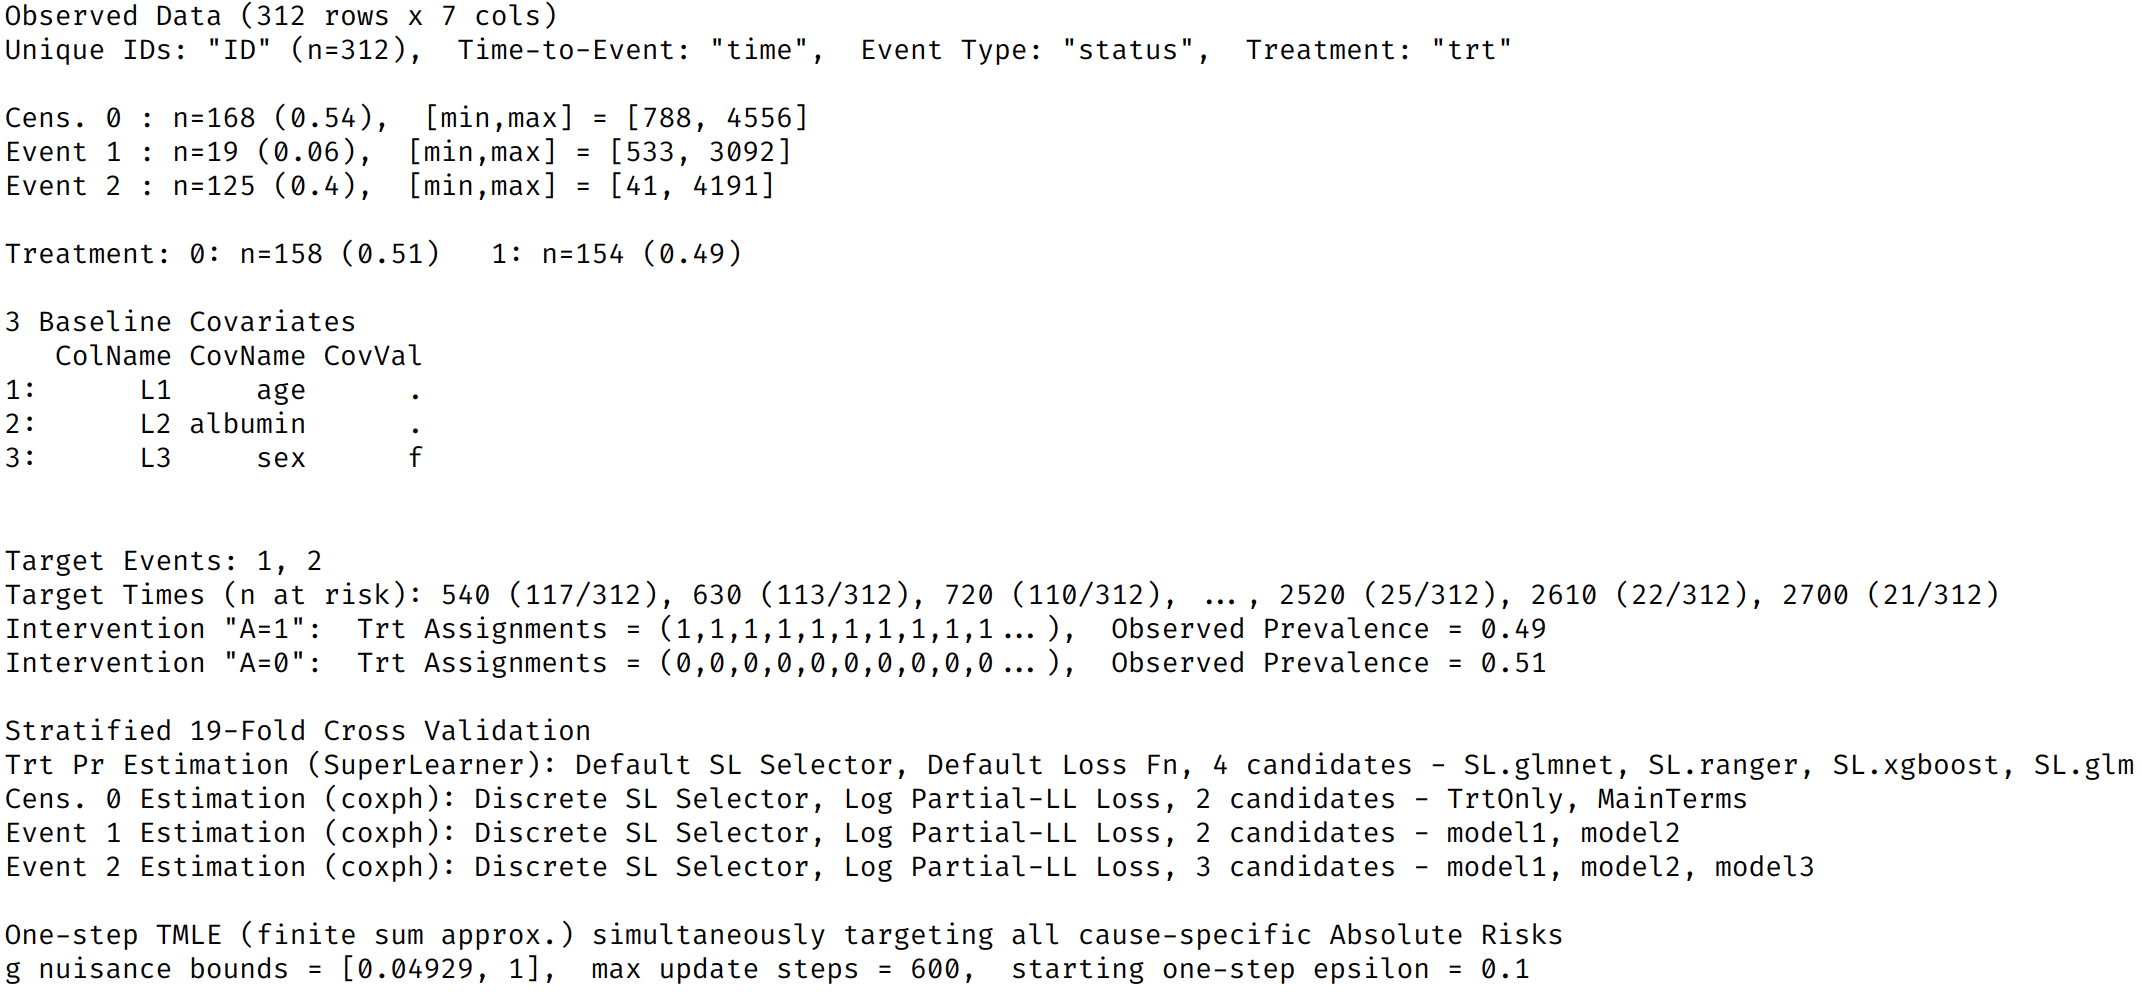
\includegraphics[width=\linewidth]{fig/ConcreteArgs.png}
\end{figure}

In particular, we can see that the target analysis is for competing risks (target events = 1, 2) under interventions "A=1" and "A=0" that assign all subjects to treated and control arms respectively. Objects in the \code{"ConcreteArgs"} environment can be interrogated directly for details about any particular aspect of the estimation specification.

\subsection{doConcrete()}
\label{doConcrete}
Adequately specified \code{"ConcreteArgs"} objects can then be passed into the \code{doConcrete()} function which will then perform the specified TMLE analysis. The output is an object of class \code{"ConcreteEst"} which contains TMLE point estimates and influence curves for the cause-specific absolute risks for each targeted event at each targeted time. If the \code{GComp} argument is set to \code{TRUE}, then a Super Learner-based g-formula plugin estimate of the targeted risks will be included in the output. 

\lstset{language=r,label= ,caption= ,captionpos=b,numbers=none,otherkeywords={}, deletekeywords={}}
\begin{lstlisting}
ConcreteEst <- doConcrete(ConcreteArgs)
\end{lstlisting}

We have previously reviewed the one-step continuous-time TMLE implementation in Section \ref{estimation}, so here we will name the non-exported functions in \code{doConcrete()} which perform each of the steps of the one-step continuous-time survival TMLE procedure, in case users wish to explore the implementation in depth.

The cross-validation (Section \ref{cv}) is checked and evaluated in \code{formatArguments()}, returning fold assignments as the \code{.[["CVFolds"]]} element of the \code{"ConcreteArgs"} object.

The initial estimation of nuisance parameters and is performed by the function \code{getInitialEstimate()} which depends on \code{getPropScore()} for propensity scores (Section \ref{trtps-est}) and \code{getHazEstimate()} for the conditional hazards (Section \ref{haz-est}).

Computing of EICs is done by \code{getEIC()} which is used within the \code{doTmleUpdate()} function which performs the one-step TMLE update procedure (Section \ref{EIC}).

\subsubsection{ConcreteEst objects}
\label{concreteest}
The print method for \code{"ConcreteEst"} objects summarizes the estimation target and displays diagnostic information about TMLE update convergence, intervention-related nuisance parameter truncation, and the nuisance parameter Super Learners.

\lstset{language=r,label= ,caption= ,captionpos=b,numbers=none,otherkeywords={}, deletekeywords={}}
\begin{lstlisting}
print(ConcreteEst, Verbose  = TRUE)
\end{lstlisting}

\begin{figure}[H]
\center
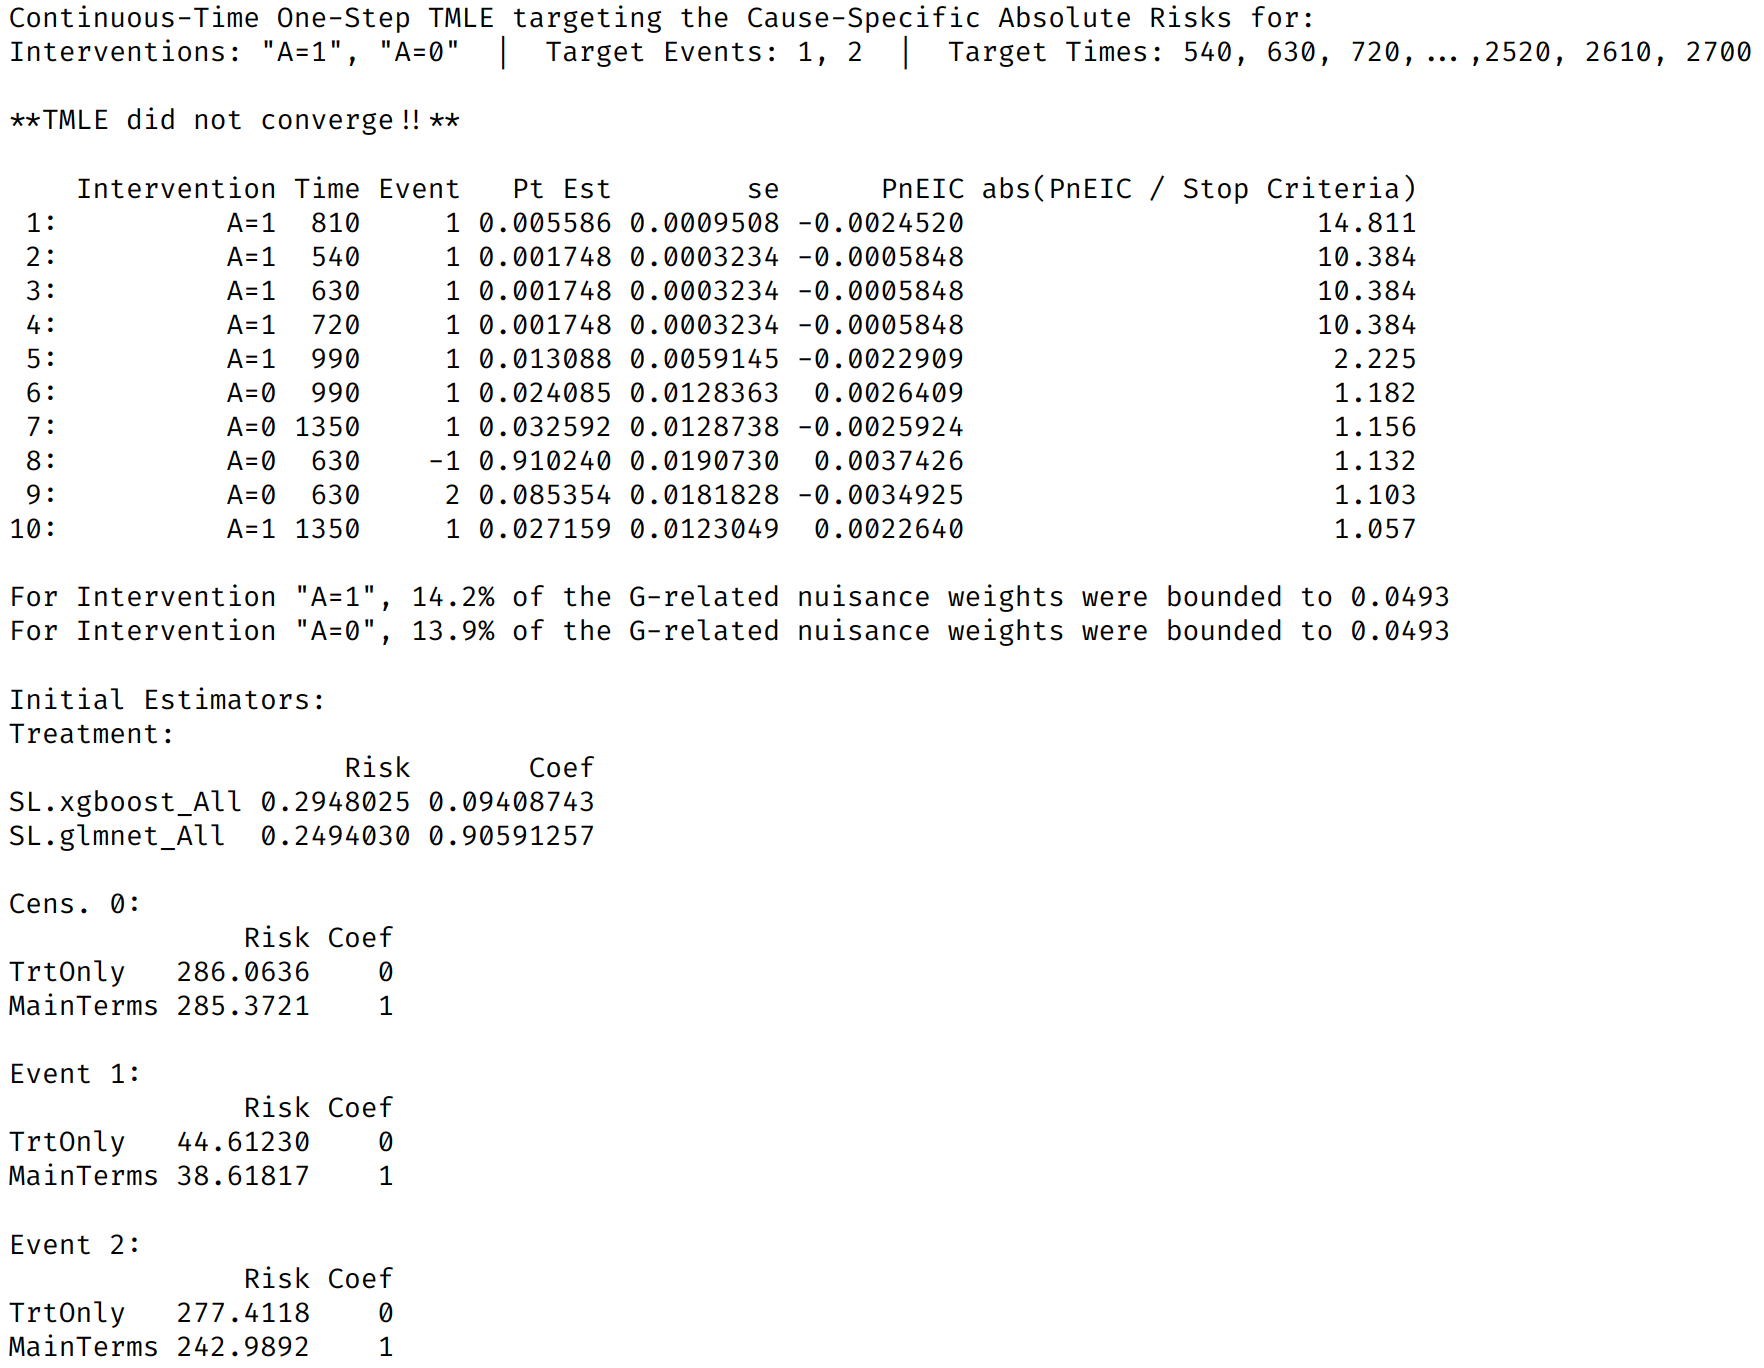
\includegraphics[width=\linewidth]{fig/ConcreteEst.png}
\end{figure}

If TMLE has not converged, the mean EICs that have not attained the desired cutoff will be displayed in a table. Convergence can be attained by increasing the maximum number of iterations, though as seen above, even very small PnEIC values may not meet the convergence criteria at target times when few events have yet occurred.

The extent of g-related nuisance parameter truncation for each intervention is also reported, both in terms of the percentage of nuisance weights that are truncated and the percentage of subjects that have truncated nuisance weights. and if users suspect possible positivity issues, the plot method for \code{"ConcreteEst"} objects can be used to visualize the distribution of estimated propensity scores for each intervention, with the red vertical line marking the cutoff for truncation.

\lstset{language=r,label= ,caption= ,captionpos=b,numbers=none,otherkeywords={}, deletekeywords={}}
\begin{lstlisting}
plot(ConcreteEst, ask  = FALSE)
\end{lstlisting}
\begin{figure}[H]
\center
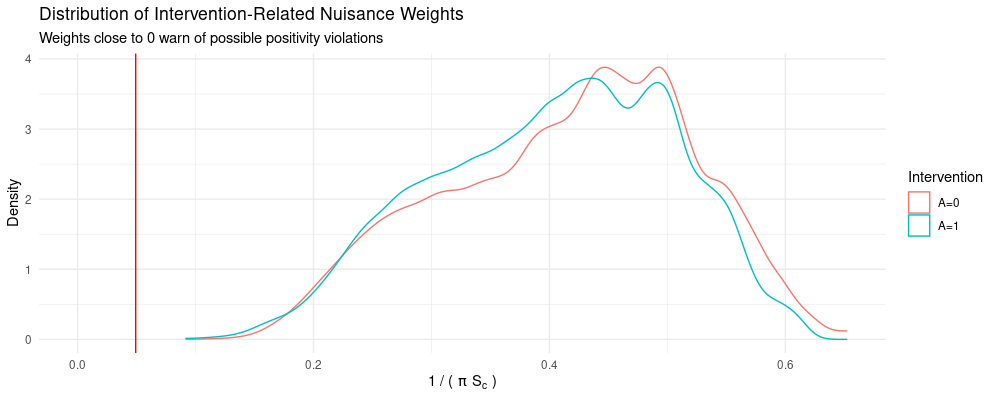
\includegraphics[width=\linewidth]{fig/ConcreteEst-PS.png}
\end{figure}

Propensity scores close to 0 indicate the possibility of positivity violations and may warrant re-examining the target time(s), interventions, and covariate adjustment sets. In typical survival applications, positivity issues may arise when targeting times at which some subjects are highly likely to have been censored, or if certain subjects are unlikely to have received a desired treatment intervention. For guidance on handling positivity issues, see \cite{petersen_diagnosing_2012}.

Lastly, the candidate estimators of nuisance parameters are summarized with the cross-validated risk of each estimator followed by their weighting in the Super Learner ensemble. 

\subsection{getOutput()}
\label{getoutput}
\code{getOutput()} takes as an argument the \code{"ConcreteEst"} object returned by \code{doConcrete()} and can be used to produce tables and plots of the cause-specific risks, risk differences, and relative risks. By default \code{getOutput()} returns a \code{data.table} with point estimates and pointwise standard errors for cause-specific absolute risks, risk differences, and risk ratios. By default, the first listed intervention is used as the "treated" group while the second is considered "control"; other contrasts can be specified via the \code{Intervention} argument. Below we show a subset of the relative risk estimates produced by the "nutshell" estimation specification for the pbc dataset. 

\lstset{language=r,label= ,caption= ,captionpos=b,numbers=none,otherkeywords={}, deletekeywords={}}
\begin{lstlisting}
ConcreteOut <- getOutput(ConcreteEst = ConcreteEst, Estimand = "RD",
			 Intervention = 1:2, GComp = TRUE, Simultaneous = TRUE, Signif = 0.05)
head(ConcreteOut, 12)
\end{lstlisting}

\begin{figure}[H]
\centering
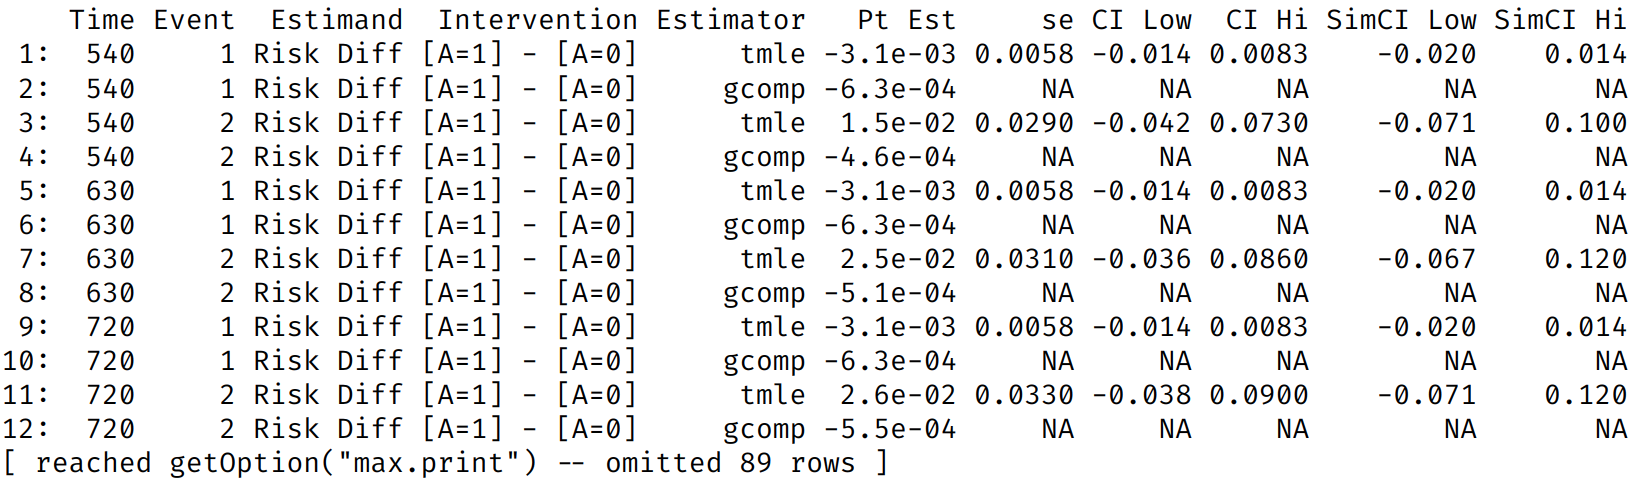
\includegraphics[width=\linewidth]{fig/rd-tbl.png}
\end{figure}

From left to right, the first five columns show the target times, target events, estimands, interventions, and estimators. The following columns show the point estimates, estimated standard error, confidence intervals and simultaneous confidence bands. Desired level of CI coverage is controlled by the \code{Signif} argument which is set to a default alpha = 0.05, and whether or not to compute a simultaneous confidence band is controlled by the \code{Simultaneous} argument.

However, as can often be the case when estimands involve many time points or multiple events, it can be difficult to quickly read treatment effects from a table. Instead plotting can make treatment effects and trends visible at a glance.

\lstset{language=r,label= ,caption= ,captionpos=b,numbers=none}
\begin{lstlisting}
plot(ConcreteOut, NullLine = TRUE, ask = FALSE)
\end{lstlisting}

\begin{figure}[H]
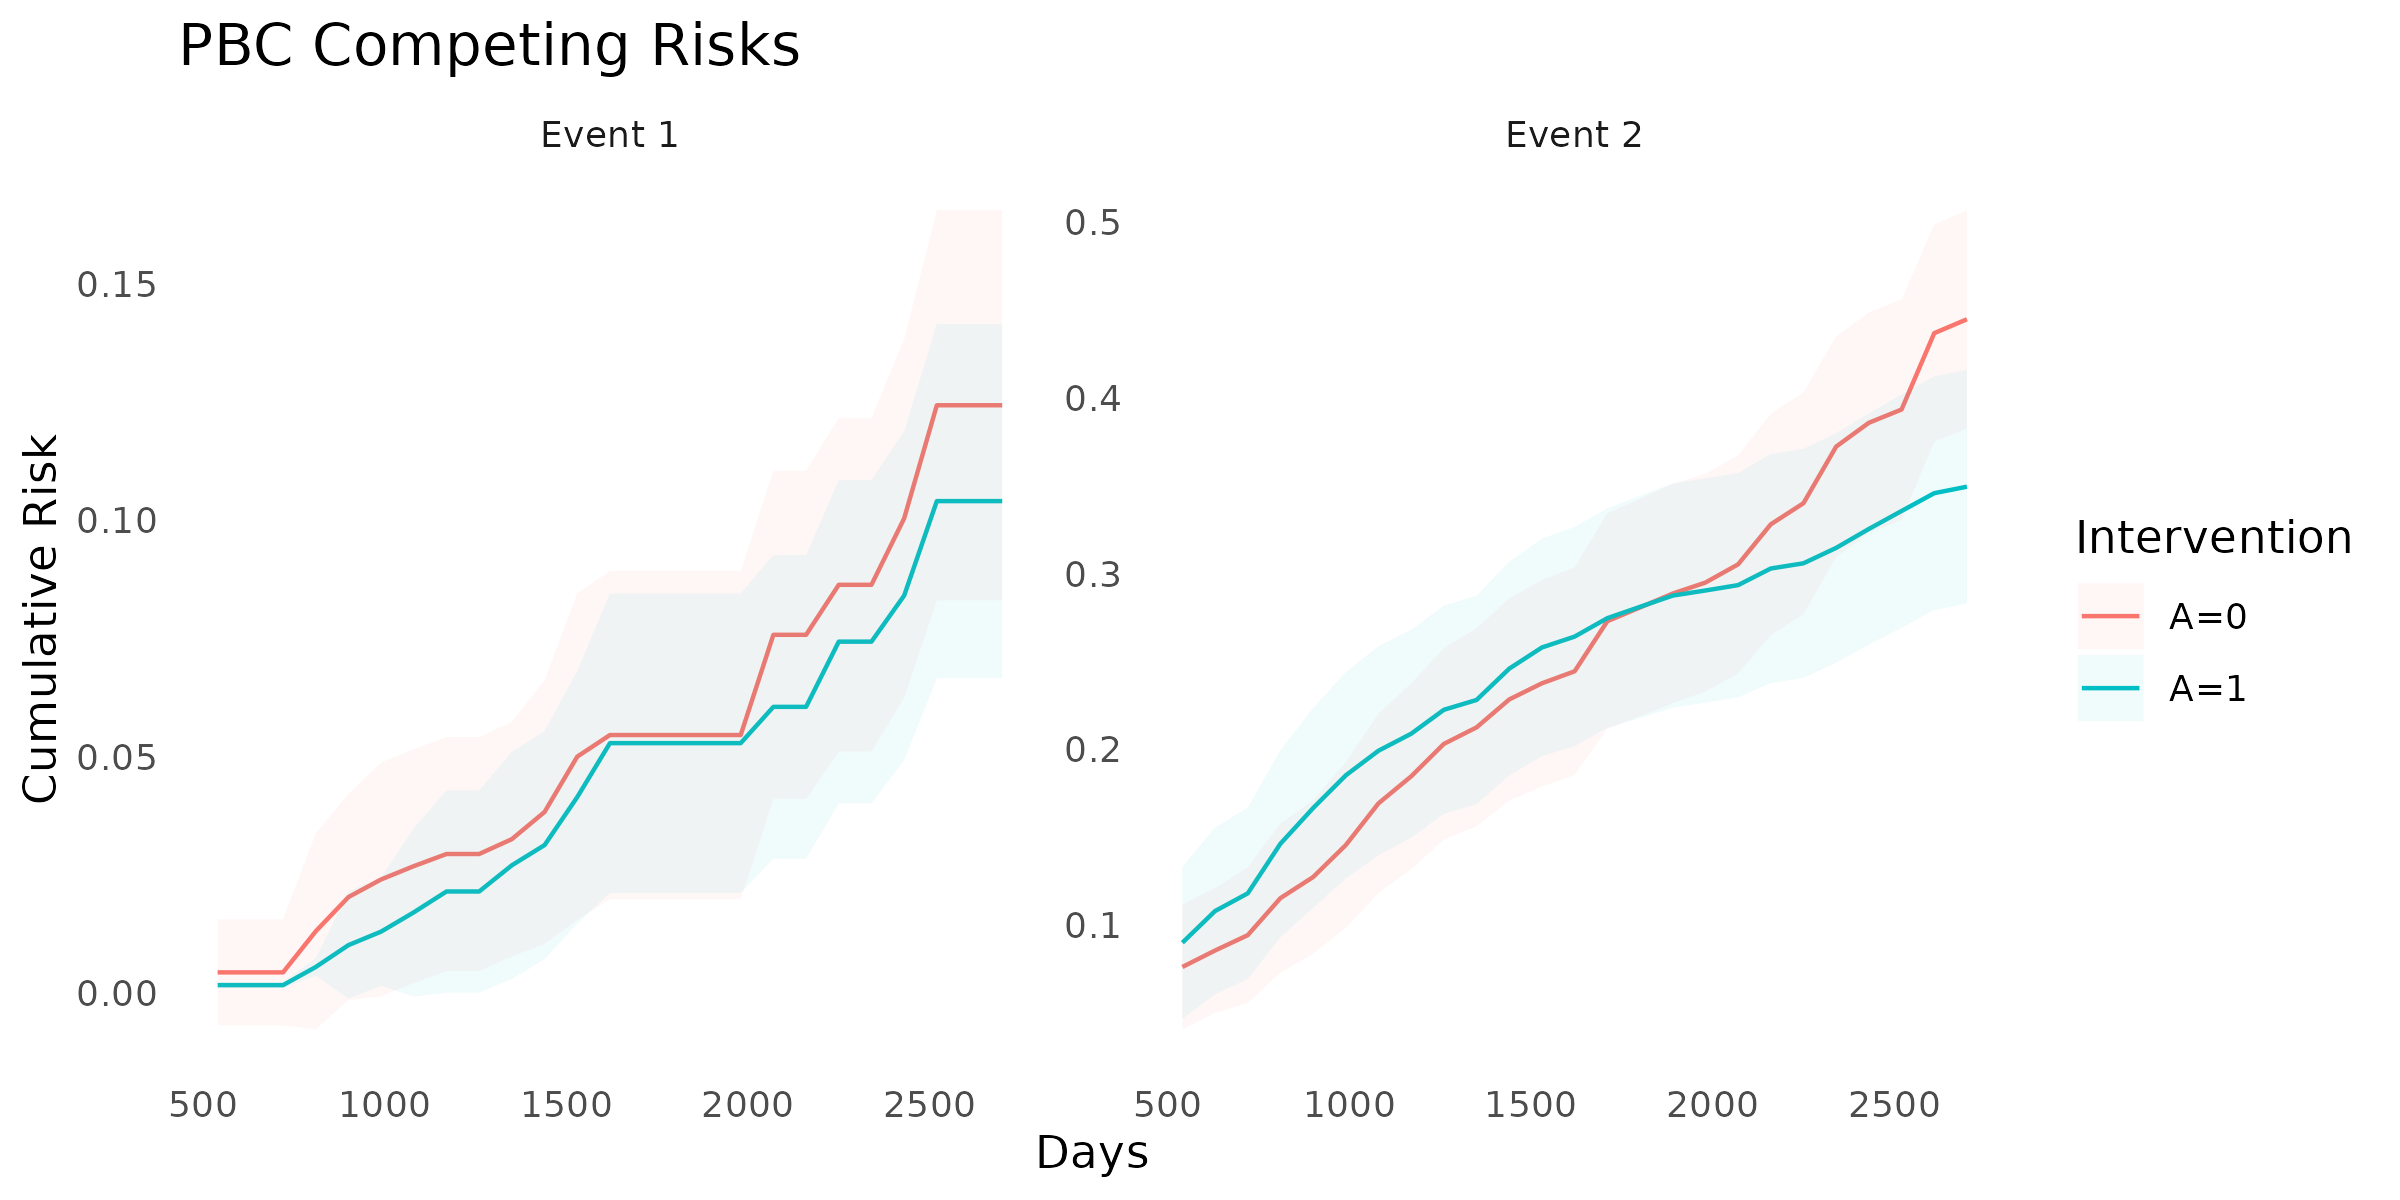
\includegraphics[width=\linewidth]{fig/concrete-pbc.png}
\end{figure}

Here 95\% confidence bands for the cause-specific risk differences across the target times is shown in grey. The \code{plot} method for \code{"ConcreteOut"} object invisibly returns a list of \code{"ggplot"} objects, which can be useful for personalizing these graphs. Currently these plots will not signal whether or not TMLE has converged and whether positivity may be an issue, so users should take care not to ignore the diagnostic output of the \code{"ConcreteEst"} object prior to obtaining effect estimates using \code{getOutput()}.

\subsection{Summary}
\label{sec:org451c014}
This paper introduces the \CRANpkg{concrete} R package implementation of continuous-time estimation for absolute risks of right-censored time-to-event outcomes. The package fits into the principled causal-inference workflow laid out by the targeted learning roadmap and allows fully compatible estimation of cause-specific absolute risk estimands for multiple events and at multiple times. The \code{formatArguments()} function is used to specify desired analyses, \code{doConcrete()} performs the specified analysis, and \code{getOutput()} is used to produce formatted output of the target estimands. Cause-specific hazards can be estimated using ensembles of proportional hazards regressions and flexible options are available for estimating treatment propensities. Confidence intervals and confidence bands can be computed for TMLEs, relying on the asymptotic linearity of the TMLEs. We are currently looking into adding support for estimating cause-specific risks using coxnet and HAL-based regressions, as well as supporting stochastic interventions with multinomial or continuous treatment variables. 


\newpage
\bibliography{main.bib}
\end{document}